\documentclass[handout, 10pt]{beamer}

%\usepackage[backend=bibtex,firstinits=true,style=verbose-inote,citestyle=authortitle]{biblatex}
\usepackage{bm}
\usepackage{graphicx}
\usepackage{subcaption}
\usepackage{amsmath}
\usepackage{amsfonts}
\usepackage{makecell}
\usepackage{filecontents}
\usepackage{biblatex}
\usepackage{xcolor}
\usepackage{subcaption}
 \newcommand{\expect}[2][]{
\ifthenelse{\equal{#1}{}}{
\mathbb{E}\left[#2\right]
}{
\underset{#1}{\mathbb{E}}\left[#2\right]
}}

\newcommand{\cov}[2][]{
\ifthenelse{\equal{#1}{}}{
\text{Cov}\left[#2\right]
}{
\underset{#1}{\text{Cov}}\left[#2\right]
}}


\newcommand{\var}[2][]{
\ifthenelse{\equal{#1}{}}{
\text{Var}[#2]
}{
\underset{#1}{\text{Var}}[#2]
}}

\newcommand{\loss}[2][]{
\ifthenelse{\equal{#1}{}}{
\mathcal{L}(#2)
}{
\mathcal{L}_{#1}(#2)
}}

\newcommand{\kl}[2]{
\text{D}_\text{KL}[#1 \parallel #2]
}

\newcommand{\R}{\mathbb{R}}
%\newcommand{\Prob}{\mathbb{P}}

\newcommand{\1}[1]{\mathds{1}\{#1\}}


%\usecolortheme{dolphin}
\setbeamertemplate{navigation symbols}{}
\setbeamertemplate{section in toc}{\inserttocsectionnumber.~\inserttocsection}

\begin{filecontents*}{references.bib}
@misc{improved_cr_for_gans,
    title={Improved Consistency Regularization for GANs},
    author={Zhengli Zhao and Sameer Singh and Honglak Lee and Zizhao Zhang and Augustus Odena and Han Zhang},
    year={2020},
    eprint={2002.04724},
    archivePrefix={arXiv},
    primaryClass={stat.ML}
}
@inproceedings{
cr_gan,
title={Consistency Regularization for Generative Adversarial Networks},
author={Han Zhang and Zizhao Zhang and Augustus Odena and Honglak Lee},
booktitle={International Conference on Learning Representations},
year={2020},
url={https://openreview.net/forum?id=S1lxKlSKPH}
}
\end{filecontents*}

\addbibresource{references.bib}


\title{Improved Consistency Regularization for GANs\footnote{\citepaper{improved_cr_for_gans}}}
%\subtitle{}
%\author{Ivan Skorokhodov}
%\date{}
%\logo{
\includegraphics[height=1cm]{images/ipavlov-logo.png}}

\newcommand{\citepaper}[1]{\citetitle{#1} by \citeauthor{#1}, \citeyear{#1}}

%\graphicspath{{./images}}

%\usetheme{lucid}
\begin{document}

\begin{frame}
    \titlepage
\end{frame}

\begin{frame}{Overview}
\begin{itemize}
    \item\pause CR-GAN (consistency regularized) proposes to add self-supervision loss to D via augmentations
    \item\pause Authors improve upon CR-GAN model in two ways:
    \begin{itemize}
        \item\pause Add augmentations on the generated images as well
        \item\pause Add self-supervision by augmenting $z$ space as well
    \end{itemize}
    \item\pause They compare with other regularization strategies (WGAN-GP, JSR, CR-GAN, etc) and show SotA results on CIFAR-10, CelebA and ImageNet
\end{itemize}

\end{frame}


\begin{frame}{Constistency Regularized GAN (CR-GAN)\footnote{\citepaper{cr_gan}}}
\begin{itemize}
    \item\pause Let $T(x)$ be an augmentation function: it takes image $x$ and produces its augmented version
    \begin{itemize}
        \item\pause For example, randomly flips it, rotates, shifts, cutouts, etc
    \end{itemize}
    \item\pause CR-GAN adds the following loss to D:
    \begin{align*}
        L_\text{cr} = \expect[p_\text{real}(x)]{\| D(x) - D(T(x)) \|_2^2},
    \end{align*}
    where $D(x)$ is the output vector before the activation in D model.
    \item\pause CR-GAN uses BigGAN as a base model, compares to other regularization strategies and shows SotA performance
    \item\pause I.e. they improve FID for ImageNet 128x128 from 8.73 to 6.66
    \item\pause The augmentation that worked the best is random flips + random shifts 
\end{itemize}
\end{frame}


\begin{frame}{Generation artifacts in CR-GAN}
Since CR-GAN applies $T(x)$ only for real data, D thinks that augmentations is a part of real distribution.
\begin{figure}
\centering
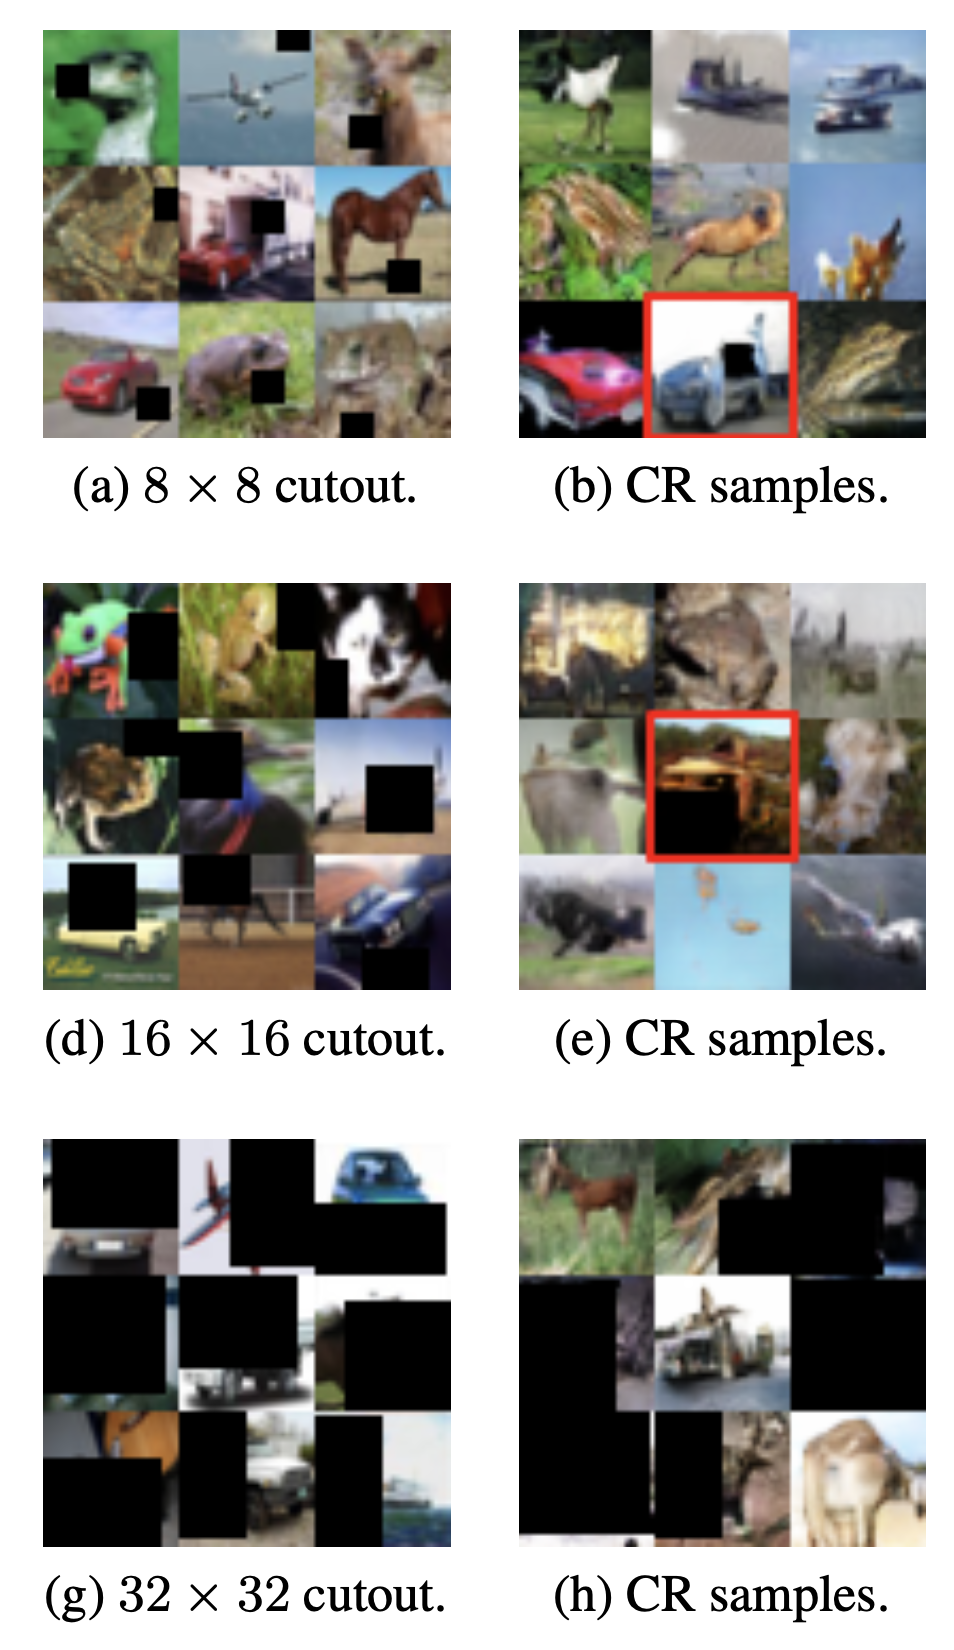
\includegraphics[width=0.3\textwidth]{images/cr-gan-generation-artifacts}
\end{figure}

\pause
This limits the set of augmentations we can use.
\end{frame}


\begin{frame}{Balanced Consistency Regularization (bCR)}
Authors remove the artifacts by adding augmentations to G as well
\begin{figure}
\centering
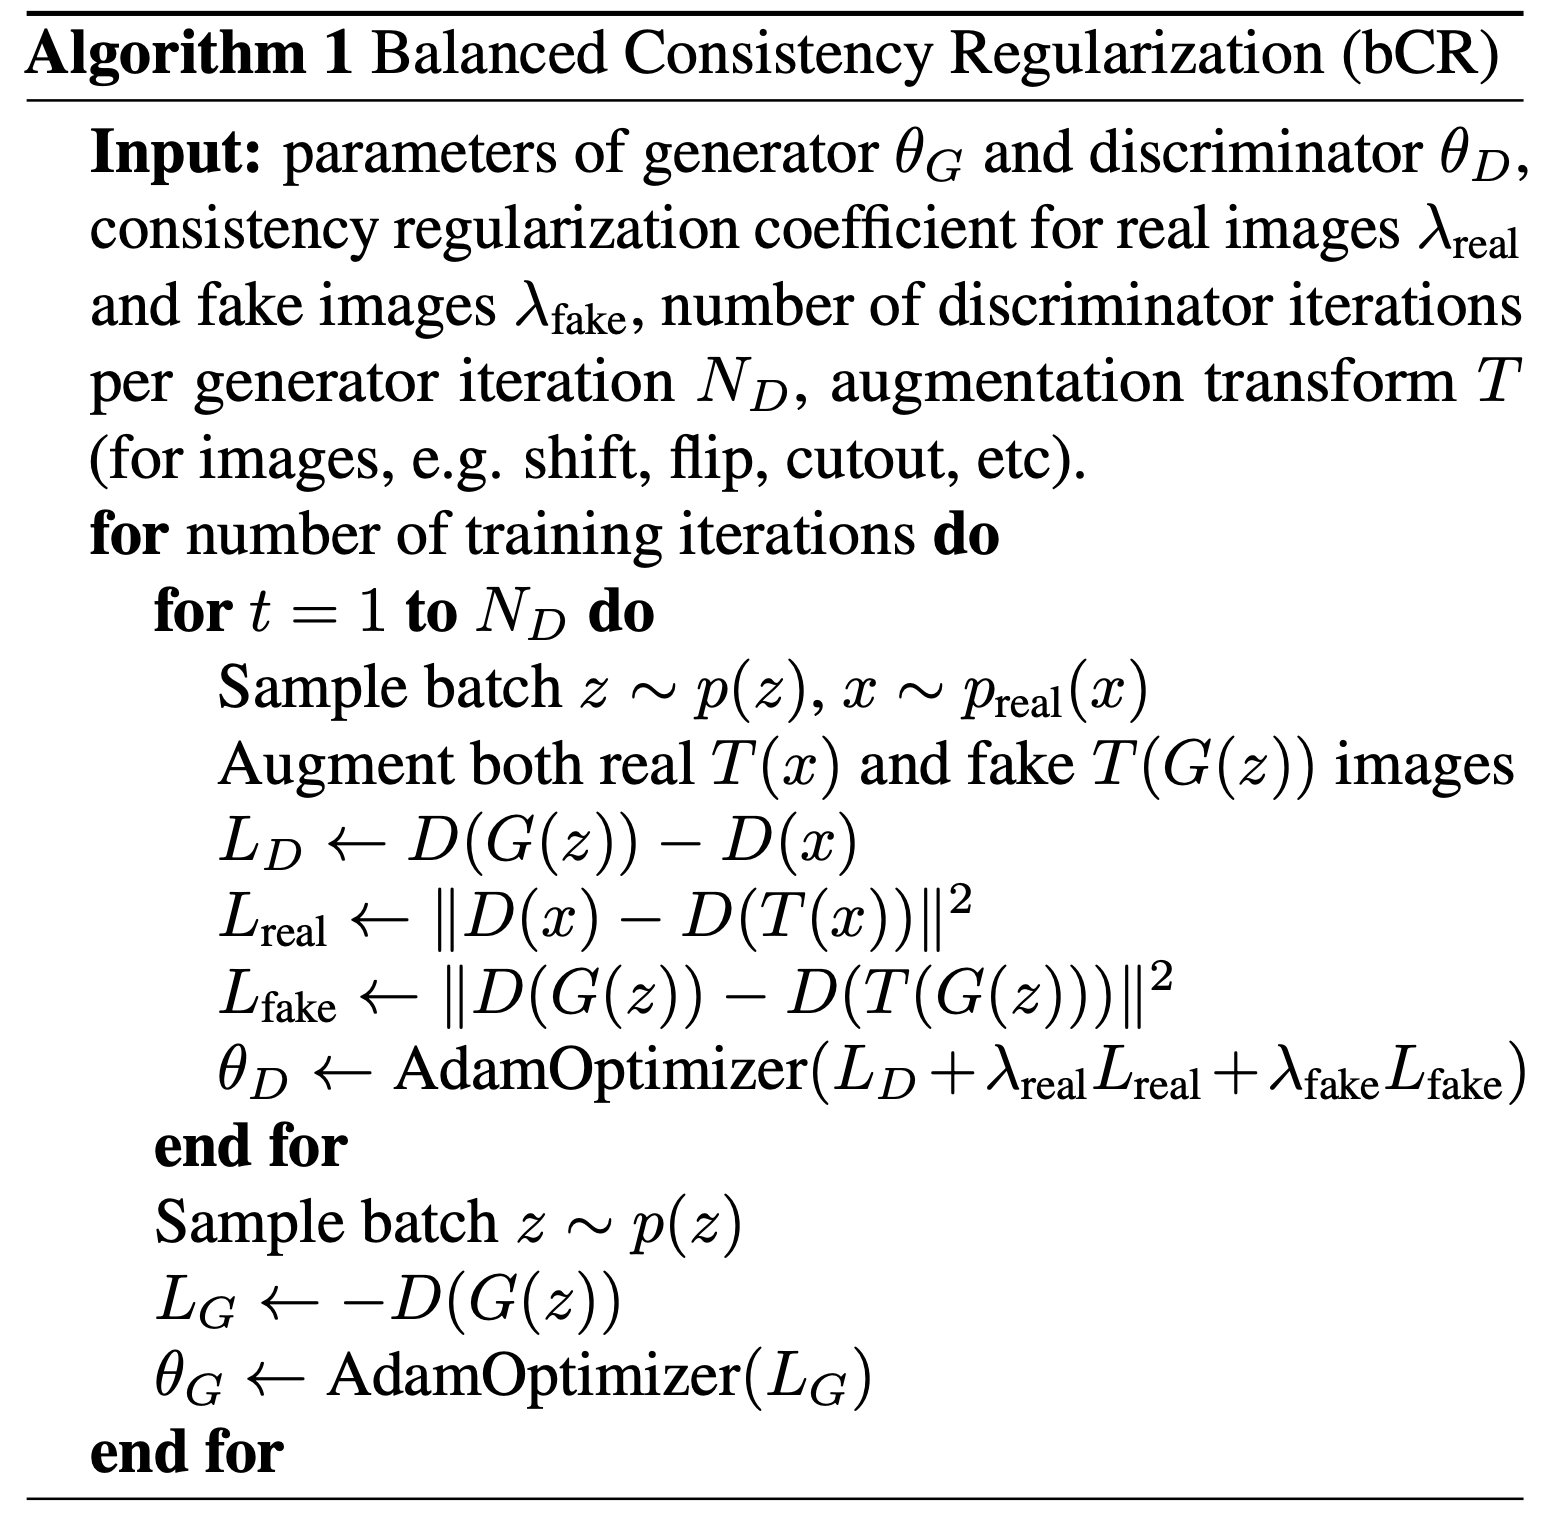
\includegraphics[width=0.6\textwidth]{images/bcr-algorithm}
\end{figure}
They usually set $\lambda_\text{real} = \lambda_\text{fake} = 10$.
\end{frame}


\begin{frame}{Latent Consistency Regularization (zCR)}
\begin{itemize}
    \item\pause Motivation: $D(G(z))$ should not change much when we change $z$ a little
    \item\pause This leads to the following additional loss
    \begin{align*}
        \| D(G(z)) - D(G(T(z))) \|_2^2
    \end{align*}
    where $T(z) = z + \varepsilon, \varepsilon \sim \mathcal{N}(0, \sigma_\varepsilon)$.
    \item\pause This loss on its own leads to mode collapse (since G tries to output same images for different $z$)
    \item\pause This problem is alleviated by forcing G to output different images for close $z$
    \begin{align*}
        - \| G(z) - G(T(z)) \|_2^2
    \end{align*}
    \item\pause This loss on G is applied with 10-20 times lower weight
\end{itemize}
\end{frame}


\begin{frame}{Results on CIFAR-10}
\begin{figure}
\centering
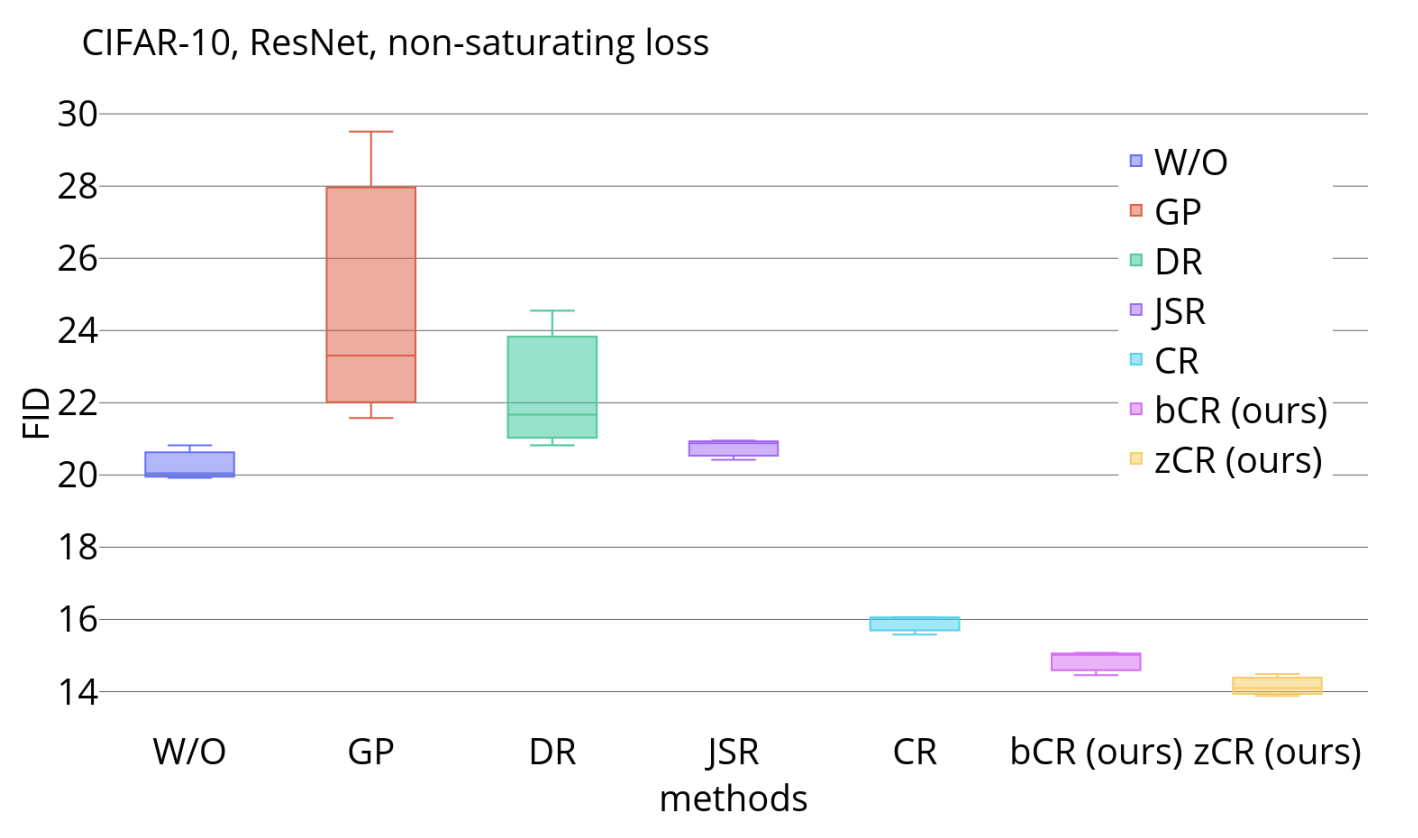
\includegraphics[width=0.8\textwidth]{images/cifar10-results.png}
\end{figure}
\end{frame}


\begin{frame}{Results on CelebA}
\begin{figure}
\centering
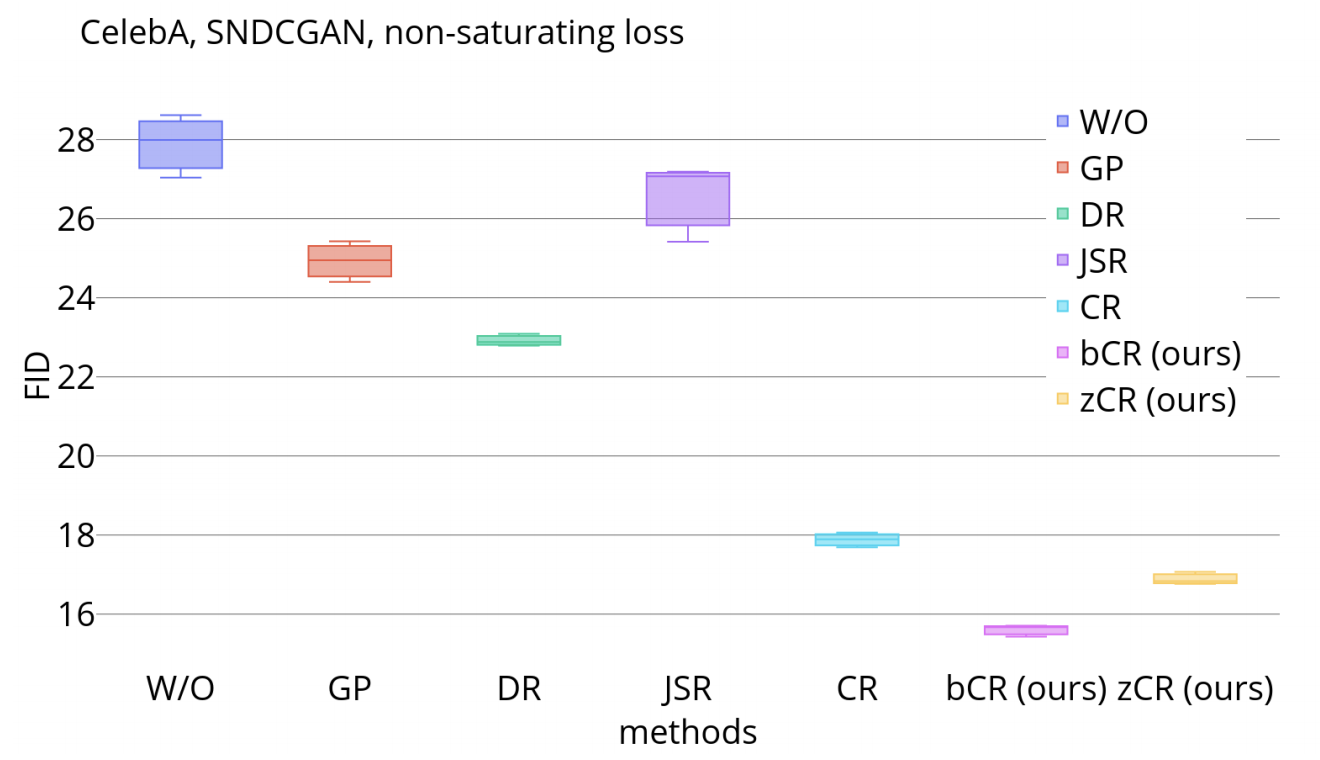
\includegraphics[width=0.8\textwidth]{images/celeba-results.png}
\end{figure}
\end{frame}


\begin{frame}{Improved CR (ICR): use bCR + zCR simultaneously}
Results for small models:
\begin{figure}
    \centering
    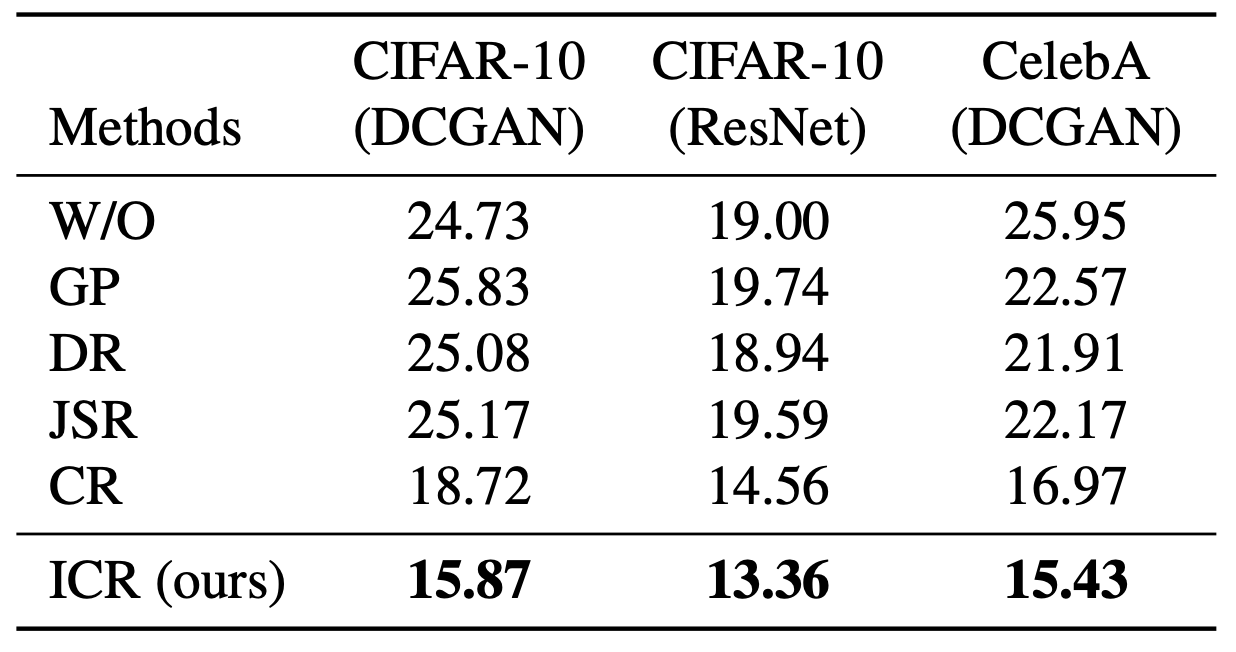
\includegraphics[width=0.5\textwidth]{images/icr-results-small-models.png}
\end{figure}

Results for BigGANs:
\begin{figure}
    \centering
    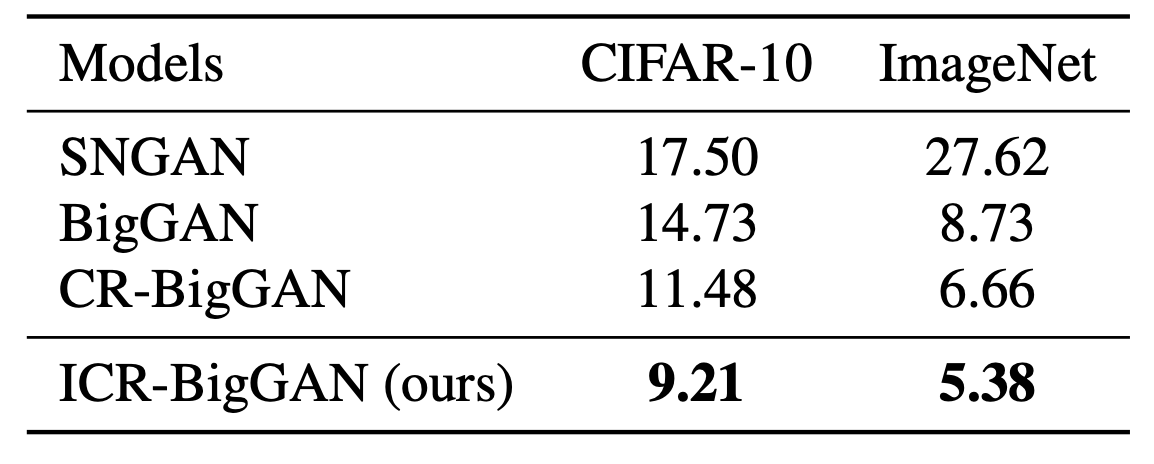
\includegraphics[width=0.4\textwidth]{images/icr-results-biggan.png}
\end{figure}
\end{frame}


\begin{frame}{bCR is not very sensitive to loss weight}
\begin{figure}
\centering
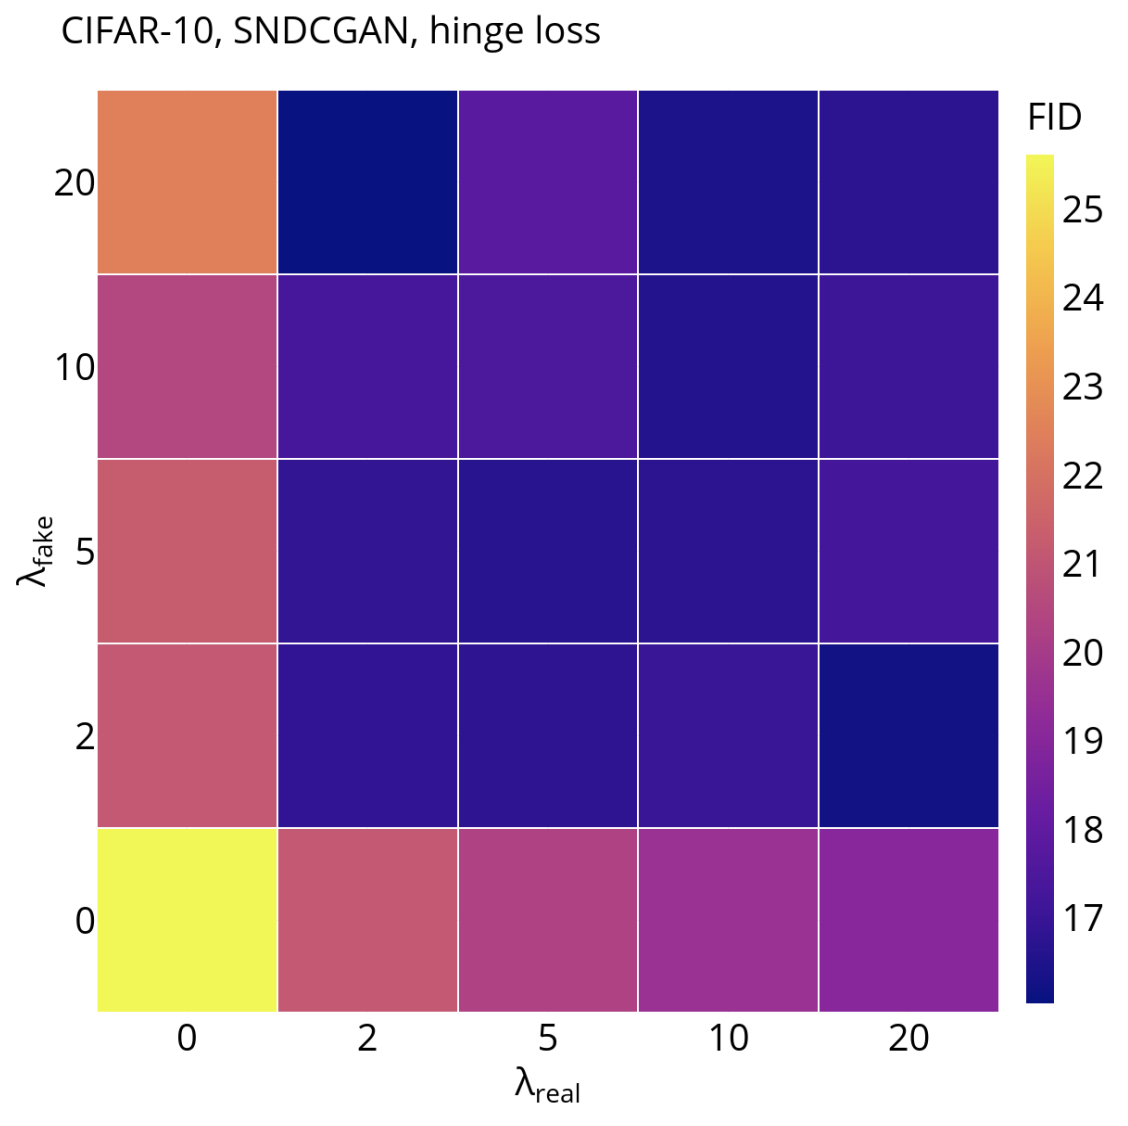
\includegraphics[width=0.5\textwidth]{images/bcr-loss-weights-sensitivity}
\caption{FID on CIFAR-10 for spectrally normalized DC-GAN}
\end{figure}
\end{frame}


\begin{frame}{Final thoughts}
\begin{itemize}
    \item\pause Number of additional forward passes for models:
    \begin{itemize}
        \item\pause CR-GAN: 1 for D
        \item\pause bCR-GAN: 2 for D
        \item\pause zCR-GAN: 1 for D, 1 for G, 1 for G inside D loop
    \end{itemize}
    \item\pause Maybe, it is possible not to apply it on each iter (aka \textit{lazy regularization} from StyleGAN2)
    \item\pause The overall direction of replacing ``math-heavy'' gradient penalties with self-supervision like losses is interesting, produces better results and trains faster
\end{itemize}
\end{frame}

\end{document}
